%!TEX program = xelatex
%!BIB program = bibtex

\documentclass[en,black,12pt,normal]{elegantnote}
\usepackage{float}
\usepackage{subfigure}
\usepackage{hyperref}


\newcommand{\upcite}[1]{\textsuperscript{\textsuperscript{\cite{#1}}}}

\title{Practical 9\\Further Analysis on GSE164805}
\author{WenYuan Jiang\\ID: 1951510}
\institute{School of Life Science, Tongji University}
%\version{1.00}
\date{\today}
\lstset{basicstyle=\footnotesize\ttfamily,frame=single,language=R}
\AtBeginEnvironment{lstlisting}{\linespread{0.75}\selectfont}

\begin{document}

\maketitle

\tableofcontents

\section{Inrtoduction}

Researchers try to identify biomarkers for early detection and effective therapy of COVID-19 patients. 
Please search a transcriptome experiment taken from COVID-19 patients as well as healthy controls. 
To interpret how the host immune system responds to the infection of sars-cov2, please perform a transcriptomics analysis.


The search and download process is done on \date{\today}.

According to the requirements, we searched in the \lstinline{GEO DataSets}, with the query \lstinline{COVID-19 patients}.

The query gives us \lstinline{2405} results, eg. \lstinline{Genome-wide DNA methylation analysis of COVID-19 severity}. 
For the convenience of further analysis, 
we narrow down the datasets to those produced by microarray (\lstinline{Expression profiling by array}).

This filter gives us two results, and we choose the \textbf{The transcriptional profiles of severe COVID-19}
as our dataset (\lstinline{Gene Expression Omnibus (GEO) and GSE164805}).\upcite{barrett2012ncbi}

The experiment is published in Front. Immunol., on 18 February 2021, 
titled \textit{Inflammation and Antiviral Immune Response Associated With Severe Progression of COVID-19}.\upcite{fimmu2021}



\section{Please perform further analysis on GSE164805\dots}

The student used \lstinline{R}, together with several packages to analysis the dataset.

\subsection{Configuring the environment}
To make the environment portable, the student uses \lstinline{Docker} to run an \lstinline{RStudio Server}. Detailed steps are shown below.

\begin{enumerate}
    \item Run \lstinline{RStudio Server} in \lstinline{Docker} using the following command.
    \begin{lstlisting}
    docker run -d -p 8787:8787 -e PASSWORD=123456 -e ROOT=TRUE -e DISABLE_AUTH=true  rocker/rstudio
    \end{lstlisting}
    \item Open the chrome and go to \lstinline{localhost:8787}.
    \item Inspect the version of the \lstinline{R}, using the following command in R shell. The output is also shown.
    \begin{lstlisting}
> version
               _                           
platform       x86_64-pc-linux-gnu         
arch           x86_64                      
os             linux-gnu                   
system         x86_64, linux-gnu           
status                                     
major          4                           
minor          0.5                         
year           2021                        
month          03                          
day            31                          
svn rev        80133                       
language       R                           
version.string R version 4.0.5 (2021-03-31)
nickname       Shake and Throw             
Warning message:
In grSoftVersion() :
  unable to load shared object '/usr/local/lib/R/modules//R_X11.so':
  libXt.so.6: cannot open shared object file: No such file or directory
    \end{lstlisting}
    \item Install the package manager \lstinline{Bioconductor}, using the following commands in R shell.
    
    \begin{lstlisting}
if (!requireNamespace("BiocManager", quietly = TRUE))
    install.packages("BiocManager")
BiocManager::install(version = "3.12")
    \end{lstlisting}
    \item Install libraries needed for the packages, input the commands in bash shell.
    
    \begin{lstlisting}
sudo apt-get install libxml2-dev libcurl4-openssl-dev curl zlib1g.dev libpng-dev
    \end{lstlisting}    
    \item Install the packages needed using the following commands in R shell.
    
    \begin{lstlisting}
BiocManager::install(c("limma","umap","GEOquery","simpleaffy","pheatmap"))
    \end{lstlisting}
    \item Be patient enough till the computer finishes all the downloading and installation. It can take several hours in the student's dormitory.
    \item Use \lstinline{library(*YourLib*)} to load a package. Run \lstinline{sessionInfo()} in R to show what packages are loaded. The following is the student's R env.
    
    \begin{lstlisting}
> sessionInfo()
R version 4.0.5 (2021-03-31)
Platform: x86_64-pc-linux-gnu (64-bit)
Running under: Ubuntu 20.04.2 LTS

Matrix products: default
BLAS/LAPACK: /usr/lib/x86_64-linux-gnu/openblas-pthread/libopenblasp-r0.3.8.so

locale:
 [1] LC_CTYPE=en_US.UTF-8       LC_NUMERIC=C              
 [3] LC_TIME=en_US.UTF-8        LC_COLLATE=en_US.UTF-8    
 [5] LC_MONETARY=en_US.UTF-8    LC_MESSAGES=C             
 [7] LC_PAPER=en_US.UTF-8       LC_NAME=C                 
 [9] LC_ADDRESS=C               LC_TELEPHONE=C            
[11] LC_MEASUREMENT=en_US.UTF-8 LC_IDENTIFICATION=C       

attached base packages:
 [1] stats4    grid      parallel  stats     graphics 
 [6] grDevices utils     datasets  methods   base     

other attached packages:
 [1] pathview_1.30.1        clusterProfiler_3.18.1
 [3] topGO_2.42.0           SparseM_1.81          
 [5] GO.db_3.12.1           graph_1.68.0          
 [7] org.Hs.eg.db_3.12.0    AnnotationDbi_1.52.0  
 [9] IRanges_2.24.1         S4Vectors_0.28.1      
[11] DOSE_3.16.0            maptools_1.1-1        
[13] sp_1.4-5               factoextra_1.0.7      
[15] ggplot2_3.3.3          FactoMineR_2.4        
[17] VennDiagram_1.6.20     futile.logger_1.4.3   
[19] pheatmap_1.0.12        umap_0.2.7.0          
[21] limma_3.46.0           GEOquery_2.58.0       
[23] Biobase_2.50.0         BiocGenerics_0.36.1   

loaded via a namespace (and not attached):
  [1] readxl_1.3.1         shadowtext_0.0.8    
  [3] backports_1.2.1      fastmatch_1.1-0     
  [5] plyr_1.8.6           igraph_1.2.6        
  [7] splines_4.0.5        BiocParallel_1.24.1 
  [9] digest_0.6.27        htmltools_0.5.1.1   
 [11] GOSemSim_2.16.1      viridis_0.6.1       
 [13] fansi_0.5.0          magrittr_2.0.1      
 [15] memoise_2.0.0        cluster_2.1.1       
 [17] openxlsx_4.2.3       Biostrings_2.58.0   
 [19] readr_1.4.0          graphlayouts_0.7.1  
 [21] matrixStats_0.59.0   askpass_1.1         
 [23] enrichplot_1.10.2    colorspace_2.0-1    
 [25] blob_1.2.1           ggrepel_0.9.1       
 [27] haven_2.4.1          xfun_0.23           
 [29] dplyr_1.0.6          RCurl_1.98-1.3      
 [31] crayon_1.4.1         jsonlite_1.7.2      
 [33] scatterpie_0.1.6     glue_1.4.2          
 [35] polyclip_1.10-0      gtable_0.3.0        
 [37] zlibbioc_1.36.0      XVector_0.30.0      
 [39] car_3.0-10           Rgraphviz_2.34.0    
 [41] abind_1.4-5          scales_1.1.1        
 [43] futile.options_1.0.1 DBI_1.1.1           
 [45] rstatix_0.7.0        Rcpp_1.0.6          
 [47] viridisLite_0.4.0    reticulate_1.20     
 [49] flashClust_1.01-2    foreign_0.8-81      
 [51] bit_4.0.4            DT_0.18             
 [53] httr_1.4.2           htmlwidgets_1.5.3   
 [55] fgsea_1.16.0         RColorBrewer_1.1-2  
 [57] ellipsis_0.3.2       XML_3.99-0.6        
 [59] pkgconfig_2.0.3      farver_2.1.0        
 [61] utf8_1.2.1           tidyselect_1.1.1    
 [63] labeling_0.4.2       rlang_0.4.11        
 [65] reshape2_1.4.4       munsell_0.5.0       
 [67] cellranger_1.1.0     tools_4.0.5         
 [69] cachem_1.0.5         downloader_0.4      
 [71] cli_2.5.0            generics_0.1.0      
 [73] RSQLite_2.2.7        broom_0.7.6         
 [75] stringr_1.4.0        fastmap_1.1.0       
 [77] bit64_4.0.5          tidygraph_1.2.0     
 [79] zip_2.2.0            purrr_0.3.4         
 [81] KEGGREST_1.30.1      ggraph_2.0.5        
 [83] formatR_1.11         KEGGgraph_1.50.0    
 [85] DO.db_2.9            leaps_3.1           
 [87] xml2_1.3.2           compiler_4.0.5      
 [89] rstudioapi_0.13      curl_4.3.1          
 [91] png_0.1-7            ggsignif_0.6.1      
 [93] tibble_3.1.2         tweenr_1.0.2        
 [95] stringi_1.6.2        RSpectra_0.16-0     
 [97] forcats_0.5.1        lattice_0.20-41     
 [99] Matrix_1.3-2         vctrs_0.3.8         
[101] pillar_1.6.1         lifecycle_1.0.0     
[103] BiocManager_1.30.15  bitops_1.0-7        
[105] data.table_1.14.0    cowplot_1.1.1       
[107] qvalue_2.22.0        R6_2.5.0            
[109] gridExtra_2.3        rio_0.5.26          
[111] lambda.r_1.2.4       MASS_7.3-53.1       
[113] assertthat_0.2.1     openssl_1.4.4       
[115] withr_2.4.2          hms_1.1.0           
[117] tidyr_1.1.3          rvcheck_0.1.8       
[119] carData_3.0-4        ggpubr_0.4.0        
[121] ggforce_0.3.3        scatterplot3d_0.3-41
[123] tinytex_0.32        
    \end{lstlisting}
\end{enumerate}

The student's hardware running the analysis is a SuperMicro Chassis with \lstinline{Xeon Gold 5117 @2.00GHz} and \lstinline{128GB DDR4@2133MHz RAM}. \textbf{For those who have an RAM less than 64GB, it may be difficult to reproduce the results of the analysis.}

\subsection{Downloading the data}

We used the \lstinline{GEOquery} package to download the expression set of \lstinline{GSE164805} and its corresponding chip data \lstinline{GPL26963}. The code below is executed in R shell to fetch the data.

\begin{lstlisting}
library(Biobase)
library(GEOquery)
library(limma)
library(umap)
library(pheatmap)
gset <- getGEO("GSE164805", GSEMatrix=TRUE, AnnotGPL=FALSE)
gpl <- getGEO("GPL26963")
\end{lstlisting}

If the Internet environment is not suitable for the download, you can manually download the data from \url{https://ftp.ncbi.nlm.nih.gov/geo/series/GSE164nnn/GSE164805/matrix/GSE164805_series_matrix.txt.gz} and \url{https://ftp.ncbi.nlm.nih.gov/geo/platforms/GPL26nnn/GPL26963/soft/GPL26963_family.soft.gz}, and extract them to a temporary directory. Use \lstinline{getGEO(filename="xxxx")} to load them.

\begin{lstlisting}
gset <- getGEO(filename = "GSE164805/GSE164805_series_matrix.txt.gz", GSEMatrix =TRUE, AnnotGPL=FALSE)
gpl <- getGEO(filename = "GSE164805/GPL26963_family.soft")
\end{lstlisting}

The loaded data should contain these columns.
\begin{lstlisting}
cols(
  ID_REF = col_character(),
  GSM5019817 = col_double(),
  GSM5019818 = col_double(),
  GSM5019819 = col_double(),
  GSM5019820 = col_double(),
  GSM5019821 = col_double(),
  GSM5019822 = col_double(),
  GSM5019823 = col_double(),
  GSM5019824 = col_double(),
  GSM5019825 = col_double(),
  GSM5019826 = col_double(),
  GSM5019827 = col_double(),
  GSM5019828 = col_double(),
  GSM5019829 = col_double(),
  GSM5019830 = col_double(),
  GSM5019831 = col_double()
)
\end{lstlisting}

\subsection{Identifying differentially expressed genes}

In this report, we only care about protein coding genes, and before we build linear models, those non-coding sequences are filtered out.

\begin{lstlisting}
gset <- gset[[1]]
coding_genes<-gpl@dataTable@table[which(gpl@dataTable@table[["TRANSCRIPT_TYPE"]]=='protein_coding'),]
ex <- exprs(gset)
ex <- ex[unlist(coding_genes['ID']),]
colnames(ex) <- c('Healthy#1','Healthy#2','Healthy#3','Healthy#4','Healthy#5','Severe#1','Severe#2','Severe#3','Severe#4','Severe#5','Mild#1','Mild#2','Mild#3','Mild#4','Mild#5')
ex <- na.omit(ex) # eliminate rows with NAs
ex <- ex[!duplicated(ex), ]  # remove duplicates
\end{lstlisting}

The following code is adapted from \lstinline{GEO2R}, used to find differentially expressed genes.
\begin{lstlisting}
# group membership for all samples
gsms <- "000001111122222"
sml <- strsplit(gsms, split="")[[1]]
qx <- as.numeric(quantile(ex, c(0., 0.25, 0.5, 0.75, 0.99, 1.0), na.rm=T))
LogC <- (qx[5] > 100) ||
  (qx[6]-qx[1] > 50 && qx[2] > 0)
if (LogC) { ex[which(ex <= 0)] <- NaN
exprs(gset) <- log2(ex) }

# assign samples to groups and set up design matrix
gs <- factor(sml)
groups <- make.names(c("healthy","mild","severe"))
levels(gs) <- groups
gset$group <- gs
design <- model.matrix(~group + 0, gset)
colnames(design) <- levels(gs)

fit <- lmFit(gset, design)  # fit linear model

# set up contrasts of interest and recalculate model coefficients
cts <- c(paste(groups[1],"-",groups[2],sep=""), paste(groups[1],"-",groups[3],sep=""), paste(groups[2],"-",groups[3],sep=""))
cont.matrix <- makeContrasts(contrasts=cts, levels=design)
fit2 <- contrasts.fit(fit, cont.matrix)

# compute statistics and table of top significant genes
fit2 <- eBayes(fit2, 0.01)
tT <- topTable(fit2, adjust="fdr", sort.by="B", number=250)

tT <- subset(tT, select=c("ID","adj.P.Val","P.Value","F","ORF","SEQUENCE","SPOT_ID"))
write.table(tT, file=stdout(), row.names=F, sep="\t")
\end{lstlisting}

The top 250 protein coding genes are stored in \lstinline{tT}, with the worst P Value of \lstinline{3.137120e-09}. All the genes' names are shown later together with their changes (3 of the 250 genes do not have a ORF name).

The quality control of the analysis can be done using Histogram of P-values.
\begin{lstlisting}
# Visualize and quality control test results.
# Build histogram of P-values for all genes. Normal test
# assumption is that most genes are not differentially expressed.
tT2 <- topTable(fit2, adjust="fdr", sort.by="B", number=Inf)
hist(tT2$adj.P.Val, col = "grey", border = "white", xlab = "P-adj",
     ylab = "Number of genes", main = "P-adj value distribution")
\end{lstlisting}
The histogram is shown below, which is our desirable result.
\begin{figure}[H]
    \centering
    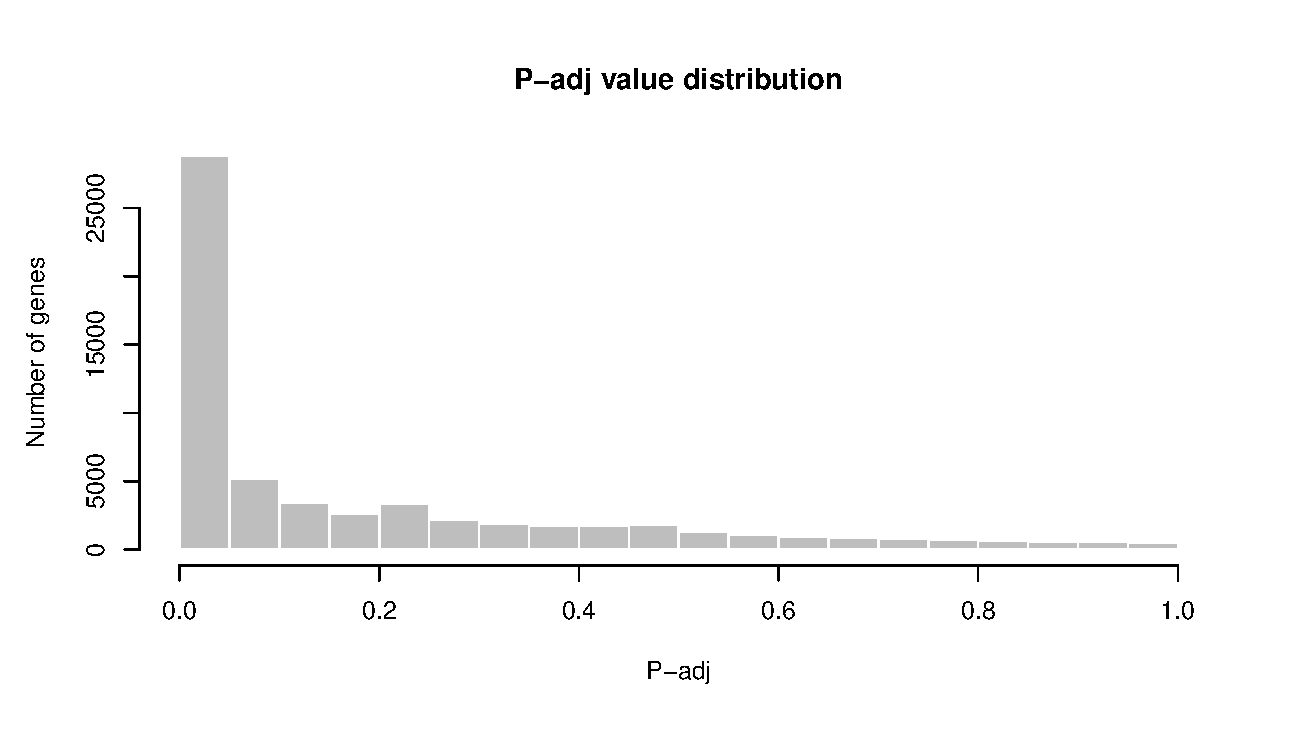
\includegraphics[width=0.9\textwidth]{image/P_Dist.eps}
    \caption{Histogram of P-values}
    \label{PValue}
\end{figure}

We summarized test results as "up", "down" or "not expressed" using the following code.
\begin{lstlisting}
# summarize test results as "up", "down" or "not expressed"
dT <- decideTests(fit2, adjust.method="fdr", p.value=0.05)
dT <- dT[row.names(tT),]
res_coding_gene<-data.frame(row.names(dT@.Data[unlist(tT['ID']),]),dT@.Data[unlist(tT['ID']),])
colnames(res_coding_gene) = c("ID","healthy.mild","healthy.severe","mild.severe")
res_coding_gene<-merge(res_coding_gene,tT[c('ID','ORF')],by = 'ID',all.x = T)
\end{lstlisting}

The genes and their changes are listed below.

\begin{lstlisting}
> write.table(res_coding_gene, file=stdout(), row.names=F, sep="\t")
"ID"	"healthy.mild"	"healthy.severe"	"mild.severe"	"ORF"
"ASHG19AP1B100010099V5"	1	1	1	"CATG00000116804.1"
"ASHG19AP1B100026912V5"	0	-1	-1	"TMEM252"
"ASHG19AP1B100044033V5"	-1	-1	1	"TMEM143"
"ASHG19AP1B100077547V5"	-1	-1	1	"TNNC2"
"ASHG19AP1B100079683V5"	-1	-1	1	"HAPLN2"
"ASHG19AP1B100095122V5"	-1	-1	0	"CATG00000062999.1"
"ASHG19AP1B100102680V5"	-1	-1	-1	"TMEM151A"
"ASHG19AP1B100132859V5"	-1	-1	0	"TMEM114"
"ASHG19AP1B100140590V5"	1	1	1	"MOS"
"ASHG19AP1B100143862V5"	1	-1	-1	"EDN1"
"ASHG19AP1B100171364V5"	-1	-1	-1	"CATG00000023238.1"
"ASHG19AP1B100197615V5"	-1	-1	-1	"TLR6"
"ASHG19AP1B100207377V5"	1	-1	-1	"TIGD3"
"ASHG19AP1B100219166V5"	-1	-1	-1	"CATG00000054736.1"
"ASHG19AP1B100226035V5"	-1	-1	1	"IRF2BP1"
"ASHG19AP1B100227479V5"	-1	-1	1	"HES5"
"ASHG19AP1B100262006V5"	-1	-1	1	"GJD3"
"ASHG19AP1B100785967V5"	-1	-1	0	"USP44"
"ASHG19AP1B100890801V5"	-1	-1	1	"SEPT12"
"ASHG19AP1B101019195V5"	-1	-1	-1	"LONRF1"
"ASHG19AP1B101133016V5"	-1	-1	1	"BEAN1"
"ASHG19AP1B101292487V5"	-1	-1	1	"SMTN"
"ASHG19AP1B101393687V5"	1	-1	-1	"BTBD19"
"ASHG19AP1B101848137V5"	-1	-1	1	"F10"
"ASHG19AP1B102078045V5"	-1	-1	1	"CNNM2"
"ASHG19AP1B102211524V5"	1	1	1	"CPA3"
"ASHG19AP1B102268874V5"	-1	-1	-1	"KIF27"
"ASHG19AP1B102926930V5"	-1	-1	-1	"FGF1"
"ASHG19AP1B102930566V5"	1	1	1	"EIF4G1"
"ASHG19AP1B102939844V5"	-1	-1	1	"PRDX1"
"ASHG19AP1B103461095V5"	0	-1	-1	"KRT2"
"ASHG19AP1B104000725V5"	-1	-1	0	"PPY"
"ASHG19AP1B104650775V5"	-1	-1	-1	"CHST1"
"ASHG19AP1B104673574V5"	-1	-1	1	"C3orf80"
"ASHG19AP1B105033128V5"	-1	-1	-1	"STRN4"
"ASHG19AP1B105392872V5"	-1	-1	1	"RPL3L"
"ASHG19AP1B106402435V5"	1	1	1	"LRRC61"
"ASHG19AP1B106458171V5"	-1	-1	0	"TEX101"
"ASHG19AP1B107974207V5"	-1	-1	-1	"LLCFC1"
"ASHG19AP1B108131779V5"	-1	-1	-1	"SAXO2"
"ASHG19AP1B108733567V5"	1	1	0	"ARHGEF9"
"ASHG19AP1B108818018V5"	-1	-1	0	"TMOD3"
"ASHG19AP1B109420977V5"	-1	-1	1	"CATG00000015125.1"
"ASHG19AP1B110408797V5"	0	-1	-1	"PGP"
"ASHG19AP1B110829606V5"	1	1	0	"TMEM106B"
"ASHG19AP1B111702966V5"	-1	-1	-1	"CATG00000039615.1"
"ASHG19AP1B112128398V5"	0	-1	-1	"KCNJ2"
"ASHG19AP1B113236502V5"	-1	-1	1	"ZNF706"
"ASHG19AP1B114603136V5"	-1	-1	0	"LCN9"
"ASHG19AP1B115327726V5"	1	-1	-1	"TULP2"
"ASHG19AP1B116099560V5"	-1	-1	-1	"CERKL"
"ASHG19AP1B116251415V5"	-1	-1	0	"CATG00000058631.1"
"ASHG19AP1B116753425V5"	-1	-1	1	"ZFP37"
"ASHG19AP1B116871577V5"	-1	-1	1	"TBCD"
"ASHG19AP1B117393755V5"	-1	-1	-1	"CATG00000028059.1"
"ASHG19AP1B118160980V5"	1	1	1	"UBXN1"
"ASHG19AP1B118570399V5"	-1	-1	-1	"RBM5"
"ASHG19AP1B119162740V5"	1	1	1	"RPS3"
"ASHG19AP1B120812793V5"	1	1	1	"CATG00000057159.1"
"ASHG19AP1B121660446V5"	-1	-1	1	"UMOD"
"ASHG19AP1B122326814V5"	-1	-1	1	"TRIM6"
"ASHG19AP1B124077767V5"	-1	-1	-1	"RALGAPA2"
"ASHG19AP1B124346093V5"	-1	-1	1	"SP140"
"ASHG19AP1B124487458V5"	0	-1	-1	"MAK"
"ASHG19AP1B124609586V5"	-1	-1	-1	"SIPA1L2"
"ASHG19AP1B126722368V5"	-1	-1	1	"PXMP4"
"ASHG19AP1B127249610V5"	-1	-1	-1	"FAM189B"
"ASHG19AP1B127343616V5"	1	1	1	"SALL2"
"ASHG19AP1B127674344V5"	-1	-1	1	"PPP1R12A"
"ASHG19AP1B127682210V5"	-1	-1	1	"ARHGEF1"
"ASHG19AP1B127764973V5"	-1	-1	1	"PSMF1"
"ASHG19AP1B130179979V5"	1	1	0	"DUSP9"
"ASHG19AP1B130926225V5"	-1	-1	1	"GLUD1"
"ASHG19AP1B131783095V5"	-1	-1	1	"ATG5"
"ASHG19AP1B132472269V5"	-1	-1	0	"RASAL2"
"ASHG19AP1B133038450V5"	1	1	1	"DUS1L"
"ASHG19AP1B133251296V5"	1	1	1	"MAGEA10"
"ASHG19AP1B134807541V5"	-1	-1	1	"GCSAML-AS1"
"ASHG19AP1B135988649V5"	-1	0	1	"EMC6"
"ASHG19AP1B136937830V5"	-1	-1	0	"IFT52"
"ASHG19AP1B139781923V5"	-1	-1	1	"ILDR1"
"ASHG19AP1B140078097V5"	1	1	0	"EXOSC2"
"ASHG19AP1B140228294V5"	-1	-1	1	"NDUFA4L2"
"ASHG19AP1B141086300V5"	-1	-1	1	"MUTYH"
"ASHG19AP1B141555700V5"	-1	-1	0	"MARCKSL1"
"ASHG19AP1B141920576V5"	-1	-1	1	"S100A16"
"ASHG19AP1B142926223V5"	0	-1	-1	"CREB3L2"
"ASHG19AP1B143197067V5"	1	1	0	"AP2M1"
"ASHG19AP1B143795176V5"	-1	-1	1	"KLK8"
"ASHG19LNC1A100002945V5"	-1	0	1	"AC092295.1"
"ASHG19LNC1A100004110V5"	-1	-1	0	"BIG-lncRNA-582"
"ASHG19LNC1A100011085V5"	-1	-1	1	"SLCO4A1-AS1"
"ASHG19LNC1A100012092V5"	-1	-1	-1	"AC069200.1"
"ASHG19LNC1A100012534V5"	-1	-1	1	"CATG00000072770.1"
"ASHG19LNC1A100015590V5"	-1	-1	0	"AC106795.3"
"ASHG19LNC1A100020163V5"	-1	-1	0	"AC006111.1"
"ASHG19LNC1A100024725V5"	1	1	0	"CATG00000011211.1"
"ASHG19LNC1A100025009V5"	-1	-1	-1	"CATG00000117297.1"
"ASHG19LNC1A100028094V5"	-1	-1	-1	"AC053513.1"
"ASHG19LNC1A100028099V5"	-1	-1	1	"AC005871.2"
"ASHG19LNC1A100032095V5"	-1	-1	0	"AC067930.1"
"ASHG19LNC1A100032333V5"	-1	-1	1	"BX255925.1"
"ASHG19LNC1A100032732V5"	0	-1	-1	"AC074132.1"
"ASHG19LNC1A100034530V5"	-1	-1	0	"ANKRD30BL"
"ASHG19LNC1A100043936V5"	0	-1	-1	"AL356356.1"
"ASHG19LNC1A100044793V5"	0	-1	-1	"AC009301.1"
"ASHG19LNC1A100048535V5"	1	-1	-1	"AC104695.2"
"ASHG19LNC1A100048539V5"	0	-1	-1	"AL590822.2"
"ASHG19LNC1A100048608V5"	-1	-1	1	"AC243585.2"
"ASHG19LNC1A100048727V5"	-1	-1	0	"TALAM1"
"ASHG19LNC1A100052346V5"	-1	-1	0	"NKX2-2-AS1"
"ASHG19LNC1A100052836V5"	-1	-1	1	"AL035696.4"
"ASHG19LNC1A100052843V5"	-1	-1	1	"LOC105370619"
"ASHG19LNC1A100057076V5"	-1	-1	-1	"CATG00000032642.1"
"ASHG19LNC1A100057683V5"	-1	-1	1	"SEC14L2"
"ASHG19LNC1A100060784V5"	0	-1	-1	"AC110769.2"
"ASHG19LNC1A100061261V5"	-1	-1	1	"CATG00000066456.1"
"ASHG19LNC1A100061364V5"	-1	-1	-1	"CATG00000084862.1"
"ASHG19LNC1A100063734V5"	0	-1	-1	"AL353616.2"
"ASHG19LNC1A100069148V5"	-1	-1	1	"CATG00000042513.1"
"ASHG19LNC1A100072148V5"	-1	-1	0	"AL161785.3"
"ASHG19LNC1A100072825V5"	1	-1	-1	"AC106028.4"
"ASHG19LNC1A100073073V5"	-1	-1	1	"CATG00000008025.1"
"ASHG19LNC1A100075651V5"	-1	-1	-1	"AL136234.1"
"ASHG19LNC1A100076086V5"	-1	-1	-1	"AC007278.2"
"ASHG19LNC1A100076220V5"	-1	-1	1	"AC046136.1"
"ASHG19LNC1A100076699V5"	-1	-1	1	"AC009088.3"
"ASHG19LNC1A100076703V5"	0	-1	-1	"AL512347.1"
"ASHG19LNC1A100080479V5"	-1	-1	1	"MEF2C-AS2"
"ASHG19LNC1A100084341V5"	-1	-1	0	"INTS6-AS1"
"ASHG19LNC1A100084701V5"	-1	-1	1	"AC005740.3"
"ASHG19LNC1A100088080V5"	-1	-1	0	"AL049651.1"
"ASHG19LNC1A100089080V5"	0	-1	-1	"AC108704.1"
"ASHG19LNC1A100092968V5"	-1	-1	1	"AL353622.2"
"ASHG19LNC1A100093030V5"	-1	-1	-1	"AC023157.3"
"ASHG19LNC1A100093161V5"	1	-1	-1	"CATG00000000010.1"
"ASHG19LNC1A100454332V5"	1	1	1	"LINC01198"
"ASHG19LNC1A100482211V5"	-1	-1	-1	"LUCAT1"
"ASHG19LNC1A100835893V5"	-1	-1	-1	"LINC00408"
"ASHG19LNC1A100854911V5"	-1	-1	1	"LINC02092"
"ASHG19LNC1A100887318V5"	-1	-1	1	"SNHG1"
"ASHG19LNC1A101254421V5"	1	1	0	"LINC01358"
"ASHG19LNC1A101637125V5"	-1	-1	-1	"DLEU2"
"ASHG19LNC1A101637126V5"	-1	-1	-1	"DLEU2"
"ASHG19LNC1A101660177V5"	-1	-1	1	"LINC01206"
"ASHG19LNC1A101683633V5"	-1	-1	1	"AC022196.1"
"ASHG19LNC1A102085612V5"	1	1	1	"AC068152.1"
"ASHG19LNC1A102092106V5"	-1	-1	0	"ADIRF-AS1"
"ASHG19LNC1A102103098V5"	-1	-1	0	"CATG00000027321.1"
"ASHG19LNC1A102428297V5"	-1	-1	-1	"DLEU2"
"ASHG19LNC1A102429018V5"	-1	-1	1	"AC012594.1"
"ASHG19LNC1A102812538V5"	1	1	1	"LINC01876"
"ASHG19LNC1A102825717V5"	-1	-1	1	"AC012594.1"
"ASHG19LNC1A102866939V5"	-1	-1	0	"AC084200.1"
"ASHG19LNC1A103685577V5"	-1	-1	1	"CATG00000004152.1"
"ASHG19LNC1A104002307V5"	1	1	0	"DANCR"
"ASHG19LNC1A104055872V5"	-1	-1	1	"AL133166.1"
"ASHG19LNC1A104444605V5"	-1	-1	1	"AC244502.1"
"ASHG19LNC1A104465952V5"	-1	-1	0	"ADIRF-AS1"
"ASHG19LNC1A104876954V5"	-1	-1	0	"CATG00000053562.1"
"ASHG19LNC1A104893279V5"	-1	-1	1	"SEMA3B"
"ASHG19LNC1A105245011V5"	-1	-1	-1	"AC073525.1"
"ASHG19LNC1A105945162V5"	-1	-1	1	"KIAA0895L"
"ASHG19LNC1A105982028V5"	-1	-1	0	"AC105935.1"
"ASHG19LNC1A106002067V5"	-1	-1	-1	"LINC01119"
"ASHG19LNC1A106013140V5"	-1	-1	1	"LINC02005"
"ASHG19LNC1A106039798V5"	-1	-1	-1	"AC009120.2"
"ASHG19LNC1A106045150V5"	-1	-1	1	"FENDRR"
"ASHG19LNC1A106399525V5"	-1	-1	1	"AL355306.2"
"ASHG19LNC1A106434347V5"	-1	-1	1	"AC103740.1"
"ASHG19LNC1A106435265V5"	-1	-1	0	"AC126696.3"
"ASHG19LNC1A106475763V5"	-1	-1	0	"CRAT"
"ASHG19LNC1A106532476V5"	1	-1	-1	"SPAG1"
"ASHG19LNC1A107535210V5"	-1	-1	0	"FAM167A-AS1"
"ASHG19LNC1A107586616V5"	-1	-1	1	"AC073529.1"
"ASHG19LNC1A107590865V5"	-1	-1	1	"Z68871.1"
"ASHG19LNC1A107597508V5"	-1	-1	-1	"N4BP2L2"
"ASHG19LNC1A107625614V5"	-1	-1	1	"AL161757.4"
"ASHG19LNC1A107787072V5"	-1	-1	-1	"MDM2"
"ASHG19LNC1A108131956V5"	-1	-1	-1	"ARMC7"
"ASHG19LNC1A108788791V5"	-1	-1	1	"NDUFA6-DT"
"ASHG19LNC1A108801755V5"	1	1	0	"SRD5A3-AS1"
"ASHG19LNC1A108832336V5"	-1	-1	0	"AC092017.4"
"ASHG19LNC1A108946762V5"	-1	-1	1	"HTRA2"
"ASHG19LNC1A109148624V5"	-1	-1	1	"LIPE-AS1"
"ASHG19LNC1A109158522V5"	1	1	1	"LINC01389"
"ASHG19LNC1A109170827V5"	-1	-1	-1	"AL034345.2"
"ASHG19LNC1A109221690V5"	1	1	1	"AC090371.2"
"ASHG19LNC1A109294555V5"	-1	-1	-1	"ANKRD13A"
"ASHG19LNC1A109427515V5"	1	1	1	"OBSCN-AS1"
"ASHG19LNC1A109552992V5"	-1	-1	-1	"RP11-782C8.5"
"ASHG19LNC1A109555842V5"	-1	-1	1	"THORLNC"
"ASHG19LNC1A109596949V5"	-1	-1	0	"AC024587.2"
"ASHG19LNC1A110168759V5"	-1	-1	0	"MEIG1"
"ASHG19LNC1A110290204V5"	-1	-1	-1	"SNHG20"
"ASHG19LNC1A110321113V5"	-1	-1	1	"GNAS"
"ASHG19LNC1A110416853V5"	1	1	0	"AL162258.1"
"ASHG19LNC1A110630287V5"	-1	-1	0	"AC105935.1"
"ASHG19LNC1A110644885V5"	-1	-1	1	"AC145207.2"
"ASHG19LNC1A111689598V5"	-1	-1	1	"TBC1D17"
"ASHG19LNC1A112100487V5"	-1	-1	1	"MKLN1-AS"
"ASHG19LNC1A112379221V5"	1	1	1	"ERAL1"
"ASHG19LNC1A113684843V5"	-1	-1	0	"SLC7A7"
"ASHG19LNC1ABL100000341V5"	-1	-1	-1	"PAX8-AS1"
"ASHG19LNC1ABL100000390V5"	1	1	0	"SOCS2-AS1"
"ASHG19LNC1ABL100000566V5"	-1	-1	-1	"LINC02366"
"ASHG19LNC1ABL100000681V5"	-1	-1	-1	"NFE4"
"ASHG19LNC1ABL100000870V5"	-1	-1	-1	"APTR"
"ASHGV40001197V5"	-1	0	1	"AC092171.1"
"ASHGV40001229V5"	1	1	1	"AC104809.2"
"ASHGV40001413V5"	-1	-1	0	"C20orf24"
"ASHGV40002118V5"	-1	-1	1	"AC244502.3"
"ASHGV40004359V5"	-1	-1	-1	"CASC18"
"ASHGV40004388V5"	1	1	1	"AC104777.1"
"ASHGV40004514V5"	-1	-1	1	"AC004233.2"
"ASHGV40006178V5"	-1	-1	1	"XLOC_008610"
"ASHGV40010017V5"	-1	-1	1	"HOXC13-AS"
"ASHGV40012850V5"	-1	-1	1	"G023046"
"ASHGV40016060V5"	-1	-1	1	"G028058"
"ASHGV40019012V5"	-1	-1	-1	"G030861"
"ASHGV40021624V5"	1	1	-1	"CCL4L2"
"ASHGV40023539V5"	-1	-1	1	"LINC02582"
"ASHGV40024194V5"	-1	-1	-1	"XLOC_013291"
"ASHGV40026229V5"	1	1	1	"G042086"
"ASHGV40027552V5"	-1	-1	-1	"LINC01920"
"ASHGV40028330V5"	1	1	0	"AC104809.2"
"ASHGV40029368V5"	-1	-1	0	"LINC01191"
"ASHGV40029603V5"	-1	0	1	"ZEB2-AS1"
"ASHGV40030424V5"	-1	-1	1	"NRSN2-AS1"
"ASHGV40033809V5"	-1	-1	-1	"LINC01639"
"ASHGV40034868V5"	-1	-1	-1	"XLOC_003243"
"ASHGV40037100V5"	1	1	1	"AC107464.1"
"ASHGV40040540V5"	0	-1	-1	"G066671"
"ASHGV40040841V5"	-1	-1	-1	"LINC01959"
"ASHGV40042878V5"	-1	-1	1	"AC008443.2"
"ASHGV40048341V5"	-1	-1	1	"LINC01393"
"ASHGV40050040V5"	0	-1	-1	"G083270"
"ASHGV40050778V5"	-1	-1	1	"G081283"
"ASHGV40051007V5"	-1	-1	1	"AP001205.1"
"ASHGV40051026V5"	1	-1	-1	"UBR5-AS1"
"ASHGV40051914V5"	0	-1	-1	"G085362"
"ASHGV40052827V5"	1	1	1	"G084493"
"ASHGV40053220V5"	-1	-1	1	"XLOC_007489"
"ASHGV40057731V5"	-1	-1	1	"MIR210HG"
"ASHGV40059259V5"	-1	-1	-1	"XLOC_001120"
"ASHGV40059449V5"	-1	-1	-1	"XLOC_005549"
"ASHGV40059791V5"	-1	-1	-1	"XLOC_013290"
"ASSPINKEIN100003643"	-1	-1	1	""
"ASSPINKEIN100008173"	-1	-1	-1	""
"ERCC-00097_63"	-1	-1	1	""              
\end{lstlisting}

Visualization of the results is shown below using \lstinline{UpSetR} Package.
\begin{figure}[H]
    \centering
    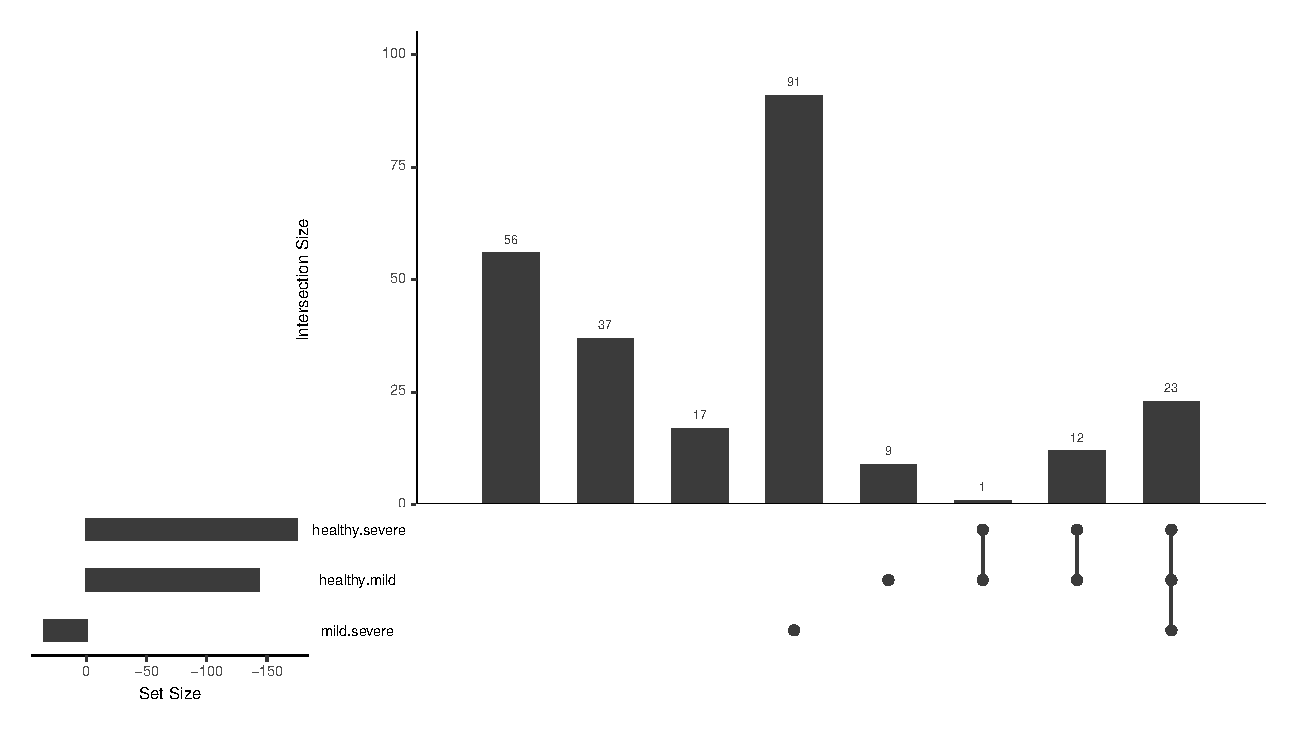
\includegraphics[width=0.9\textwidth]{image/USET.eps}
    \caption{Numbers of differentially expressed genes}
    \label{PValue}
\end{figure}

\begin{figure}[H]
    \centering
    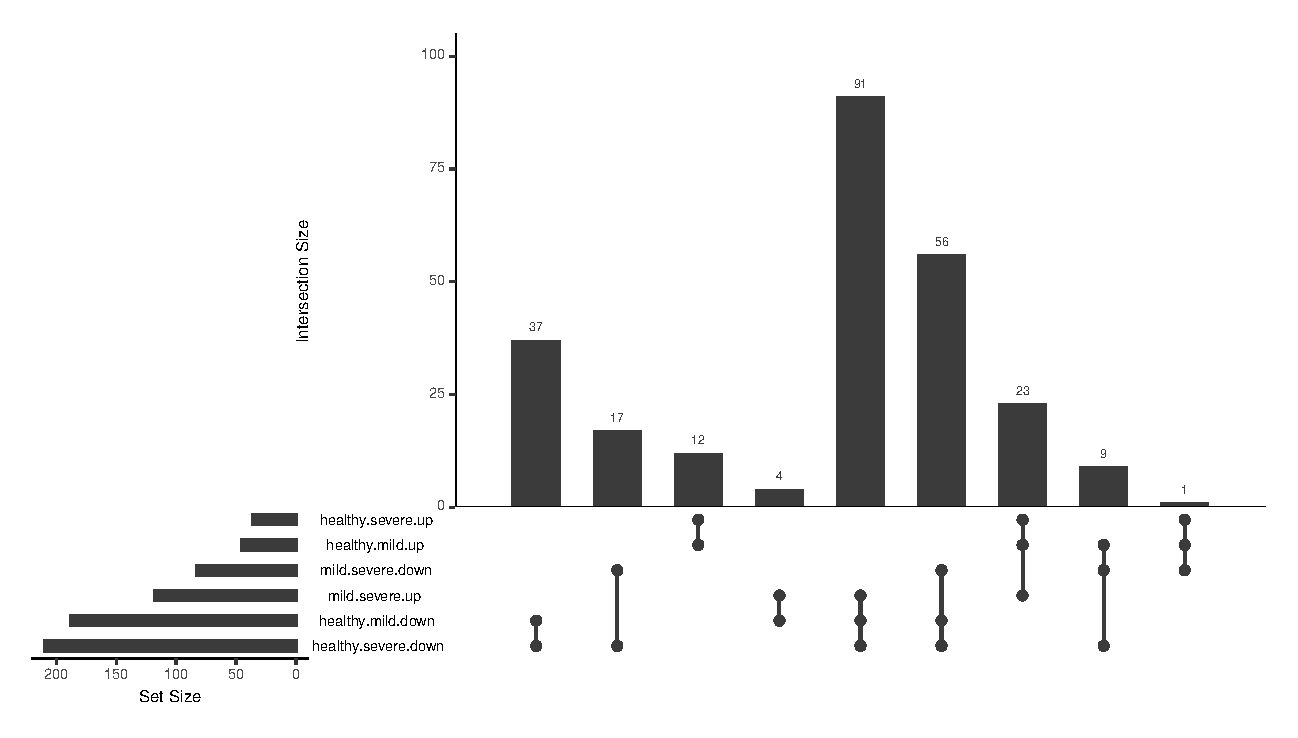
\includegraphics[width=0.9\textwidth]{image/USET2.eps}
    \caption{Numbers of up/down expressed genes}
    \label{PValue}
\end{figure}


\subsection{Principal Component Analysis \& Umap}
We performed Dimension Reduction to the expression data to study whether the data are well distributed. PCA(Principal Component Analysis) and Umap are common ways to do Dimension Reduction and data visualization.

\subsubsection{Principal Component Analysis}

The code used to perform Principal Component Analysis is shown below.

\begin{lstlisting}
library("FactoMineR")
library("factoextra")
res.pca <- PCA(t(ex))
fviz_pca_ind(res.pca, col.ind = c('Healthy','Healthy','Healthy','Healthy','Healthy','Severe','Severe','Severe','Severe','Severe','Mild','Mild','Mild','Mild','Mild'),palette = c("#00AFBB", "#E7B800", "#FC4E07"),repel = TRUE)
\end{lstlisting}

The result of PCA is shown in the figure below.
\begin{figure}[H]
    \centering
    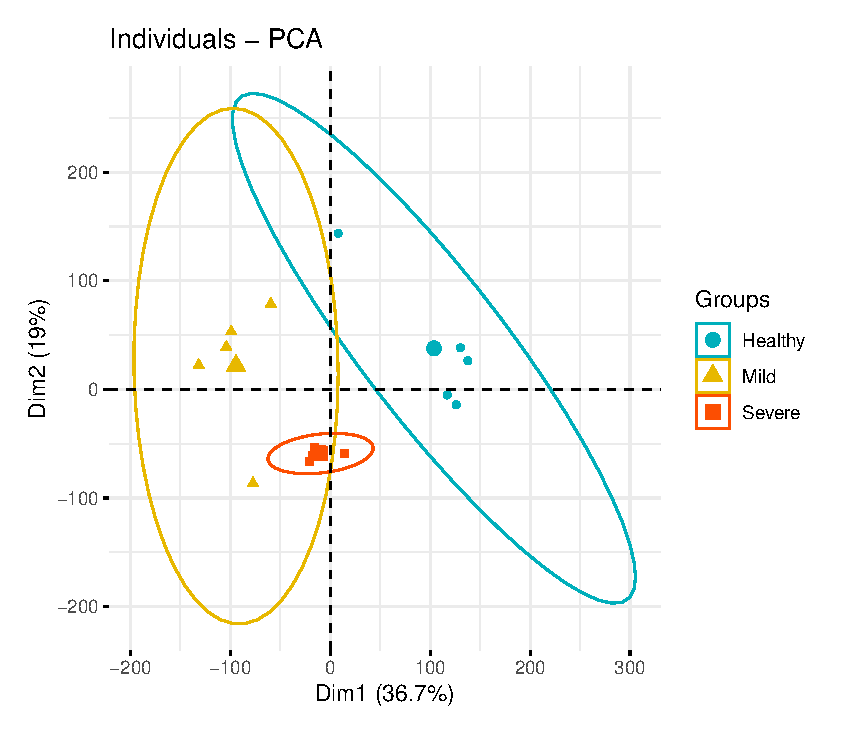
\includegraphics[width=0.7\textwidth]{image/PCA.eps}
    \caption{PCA Results}
    \label{PCA}
\end{figure}

\subsubsection{Umap}

The code used to draw umap is adapted from \lstinline{GEO2R}.

\begin{lstlisting}
ex <- na.omit(ex) # eliminate rows with NAs
ex <- ex[!duplicated(ex), ]  # remove duplicates
ump <- umap(t(ex), n_neighbors = 7, random_state = 123)
par(mar=c(3,3,2,6), xpd=TRUE)
plot(ump$layout, main="UMAP plot, nbrs=7", xlab="", ylab="", col=gs, pch=20, cex=1.5)
legend("topright", inset=c(-0.15,0), legend=levels(gs), pch=20,
       col=1:nlevels(gs), title="Group", pt.cex=1.5)
library("maptools")  # point labels without overlaps
pointLabel(ump$layout, labels = rownames(ump$layout), method="SANN", cex=0.6)
\end{lstlisting}

The umap is shown in the figure below.
\begin{figure}[H]
    \centering
    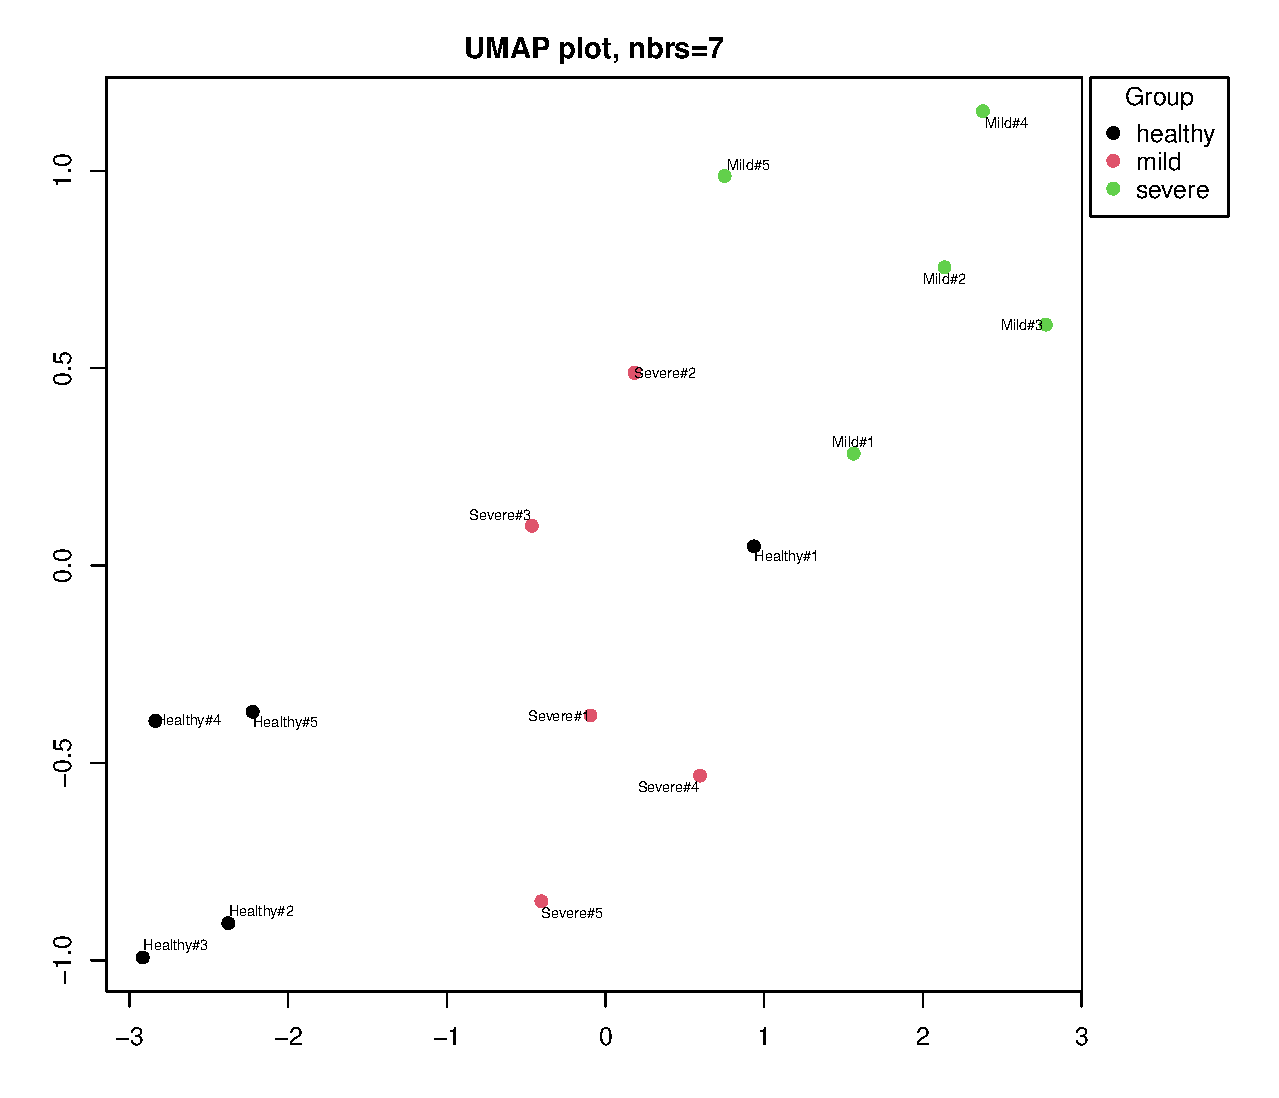
\includegraphics[width=0.7\textwidth]{image/umap.eps}
    \caption{UMap Results}
    \label{UMAP}
\end{figure}

\subsection{Visualization: Heat map}

Here we used the \lstinline{pheatmap} package to draw the heat map of all coding genes and the top 250 coding genes.

\begin{lstlisting}
pheatmap(scale(ex),border=F,show_rownames=F,show_colnames=T,legend = T)
pheatmap(scale(ex[row.names(tT),]),border=F,show_rownames=F,show_colnames=T,legend = T)
\end{lstlisting}
\begin{figure}[H]
    \centering
    \subfigure[all coding genes] {\includegraphics[width=.45\textwidth]{image/PHA.eps}}
	\subfigure[top 250 coding genes] {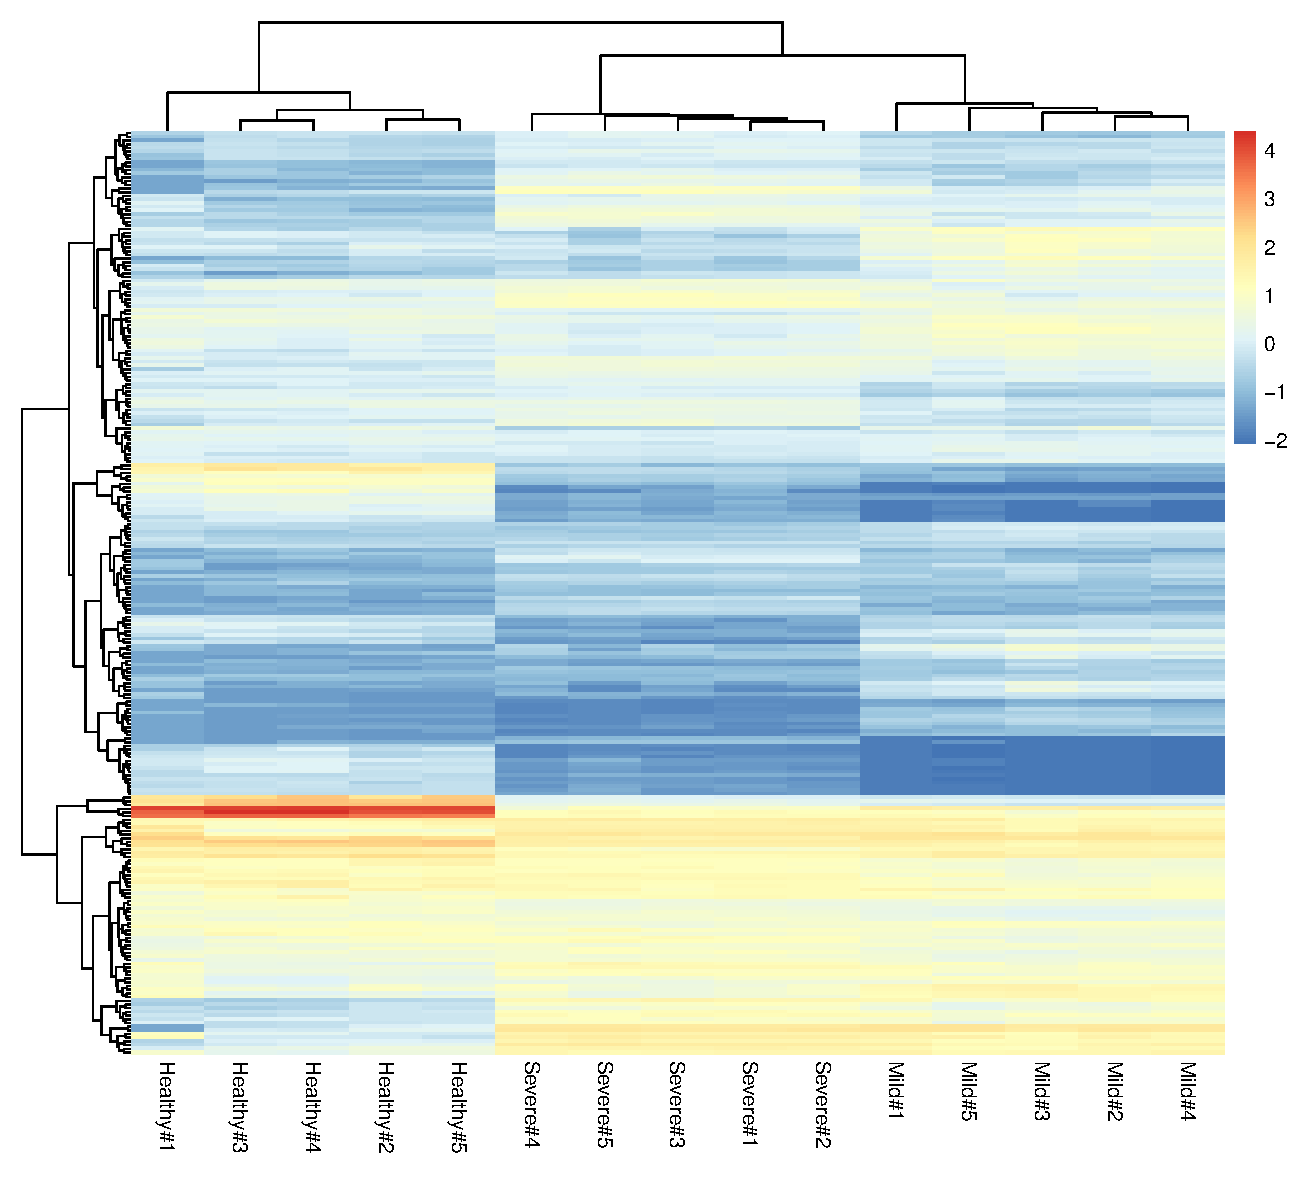
\includegraphics[width=.45\textwidth]{image/PHC.eps}}
    \caption{Heat map}
    \label{UMAP}
\end{figure}

\subsection{Visualization: GO enrichment dot plot}

The GO enrichment is done using \lstinline{DOSE, org.Hs.eg.db, topGO, clusterProfiler}.
The code belwo is an example.
\begin{lstlisting}
library(DOSE)
library(org.Hs.eg.db)
library(topGO)
library(clusterProfiler)
library(pathview)
dt<- data.frame(dT@.Data)
up_HM_genes <- coding_genes[which(coding_genes$ID %in% row.names(dt[which(dt$healthy.mild==1),])),]$ORF
up_HM_genes <- bitr(up_HM_genes, fromType="SYMBOL", toType=c("ENSEMBL", "ENTREZID"), OrgDb="org.Hs.eg.db")
ego_MF <- enrichGO(gene = up_HM_genes$ENTREZID,OrgDb = org.Hs.eg.db,ont = "MF", pAdjustMethod = "BH",pvalueCutoff = 1,qvalueCutoff = 1,readable = FALSE)
dotplot(ego_MF,title="EnrichmentGO_Health.vs.Mild_Up")
\end{lstlisting}

\begin{figure}[H]
    \centering
    \subfigure[healthy vs mild up genes] {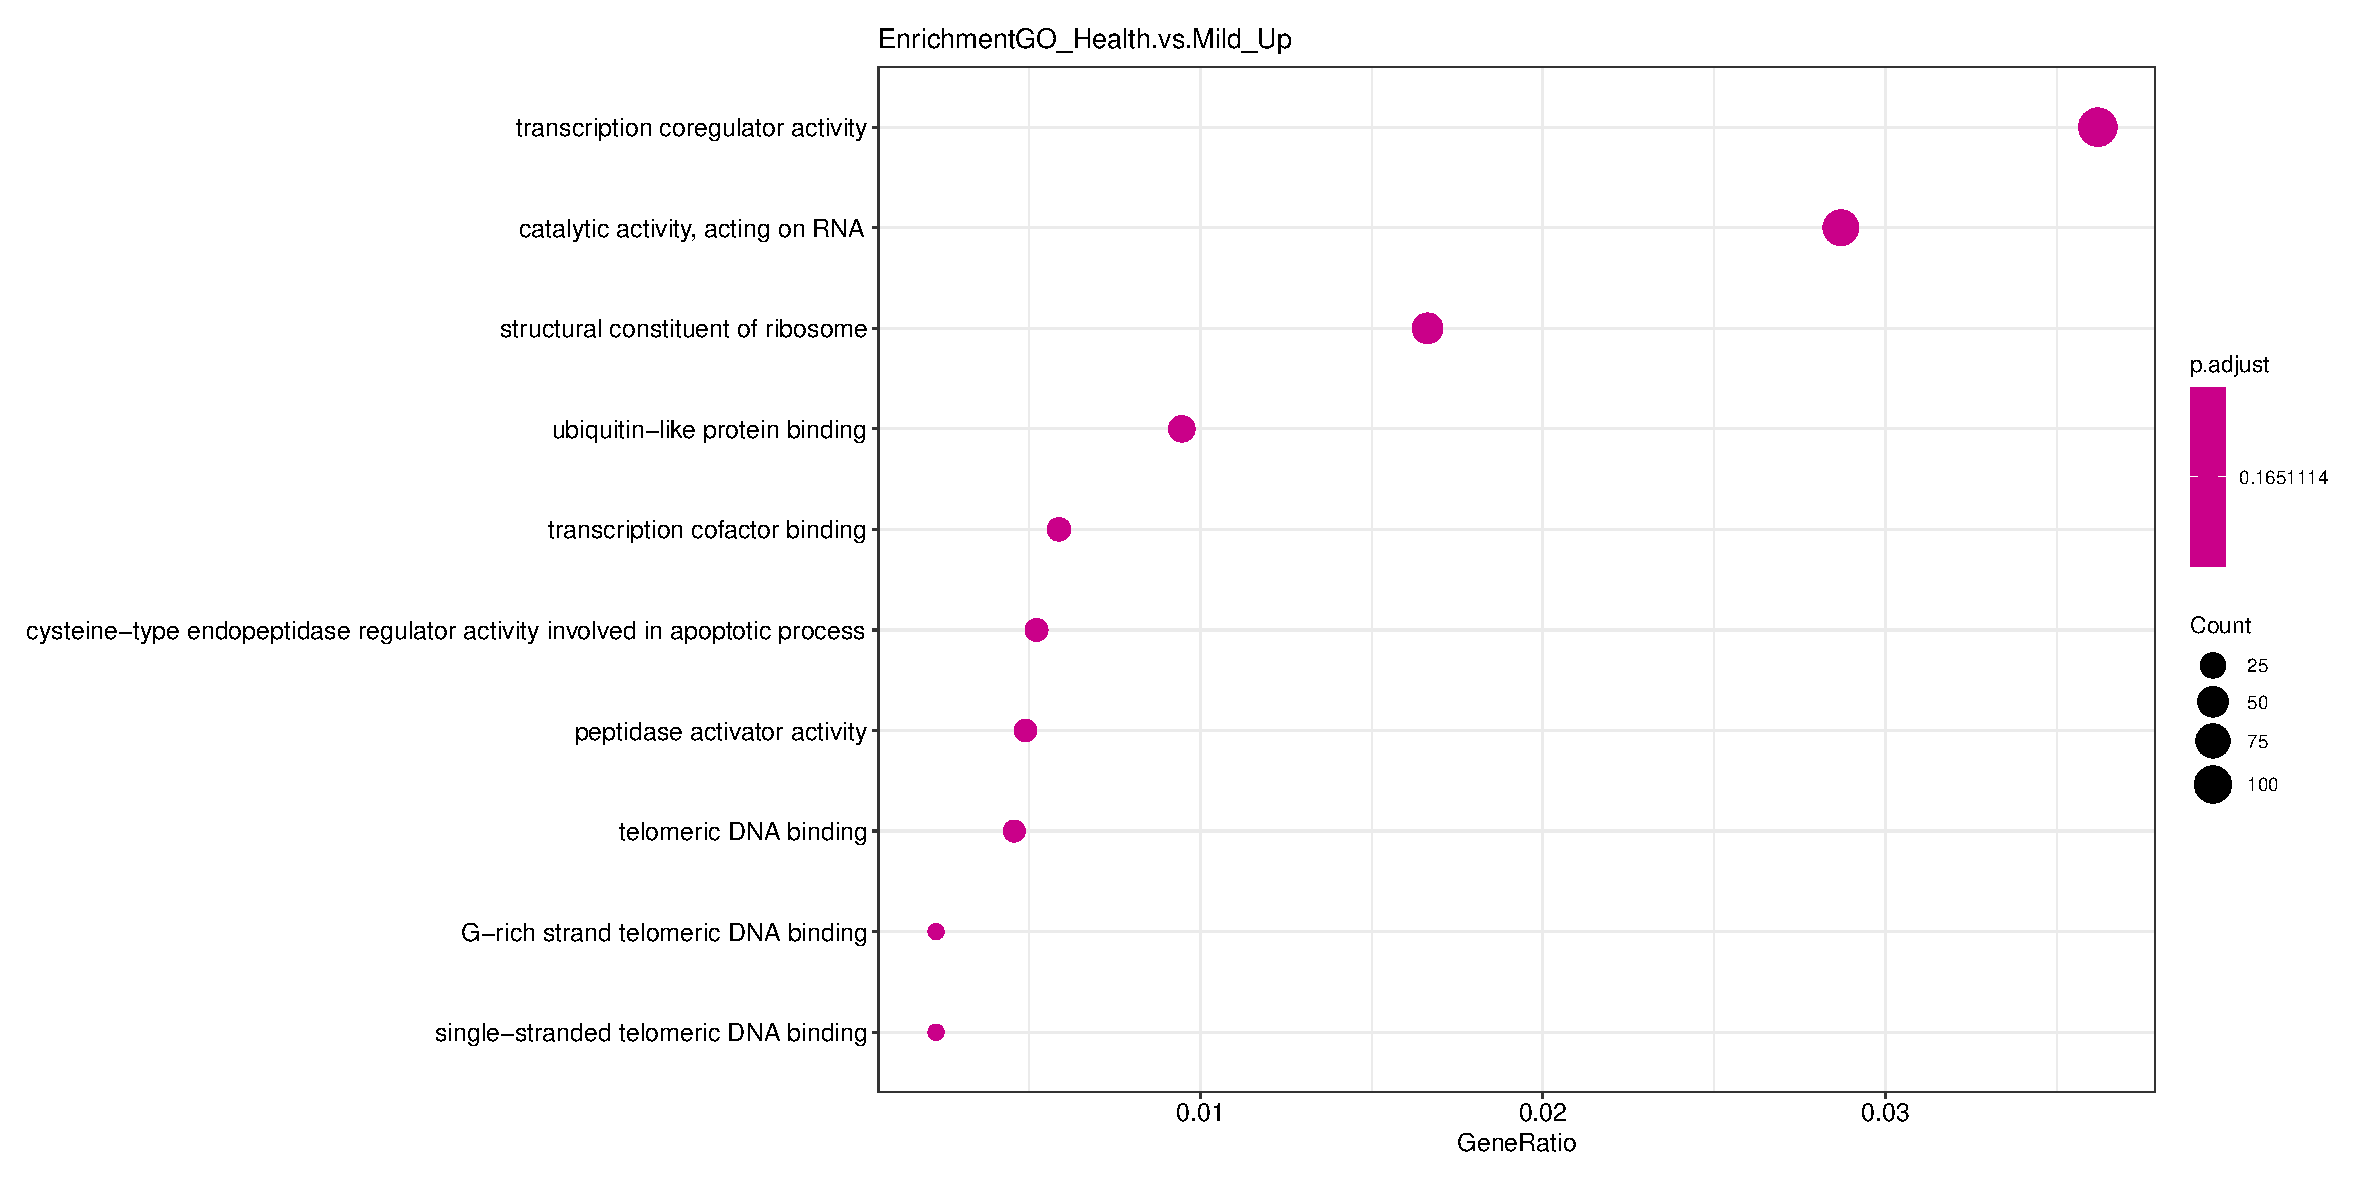
\includegraphics[width=.45\textwidth]{image/EGOHMU.eps}}
	\subfigure[healthy vs mild down genes] {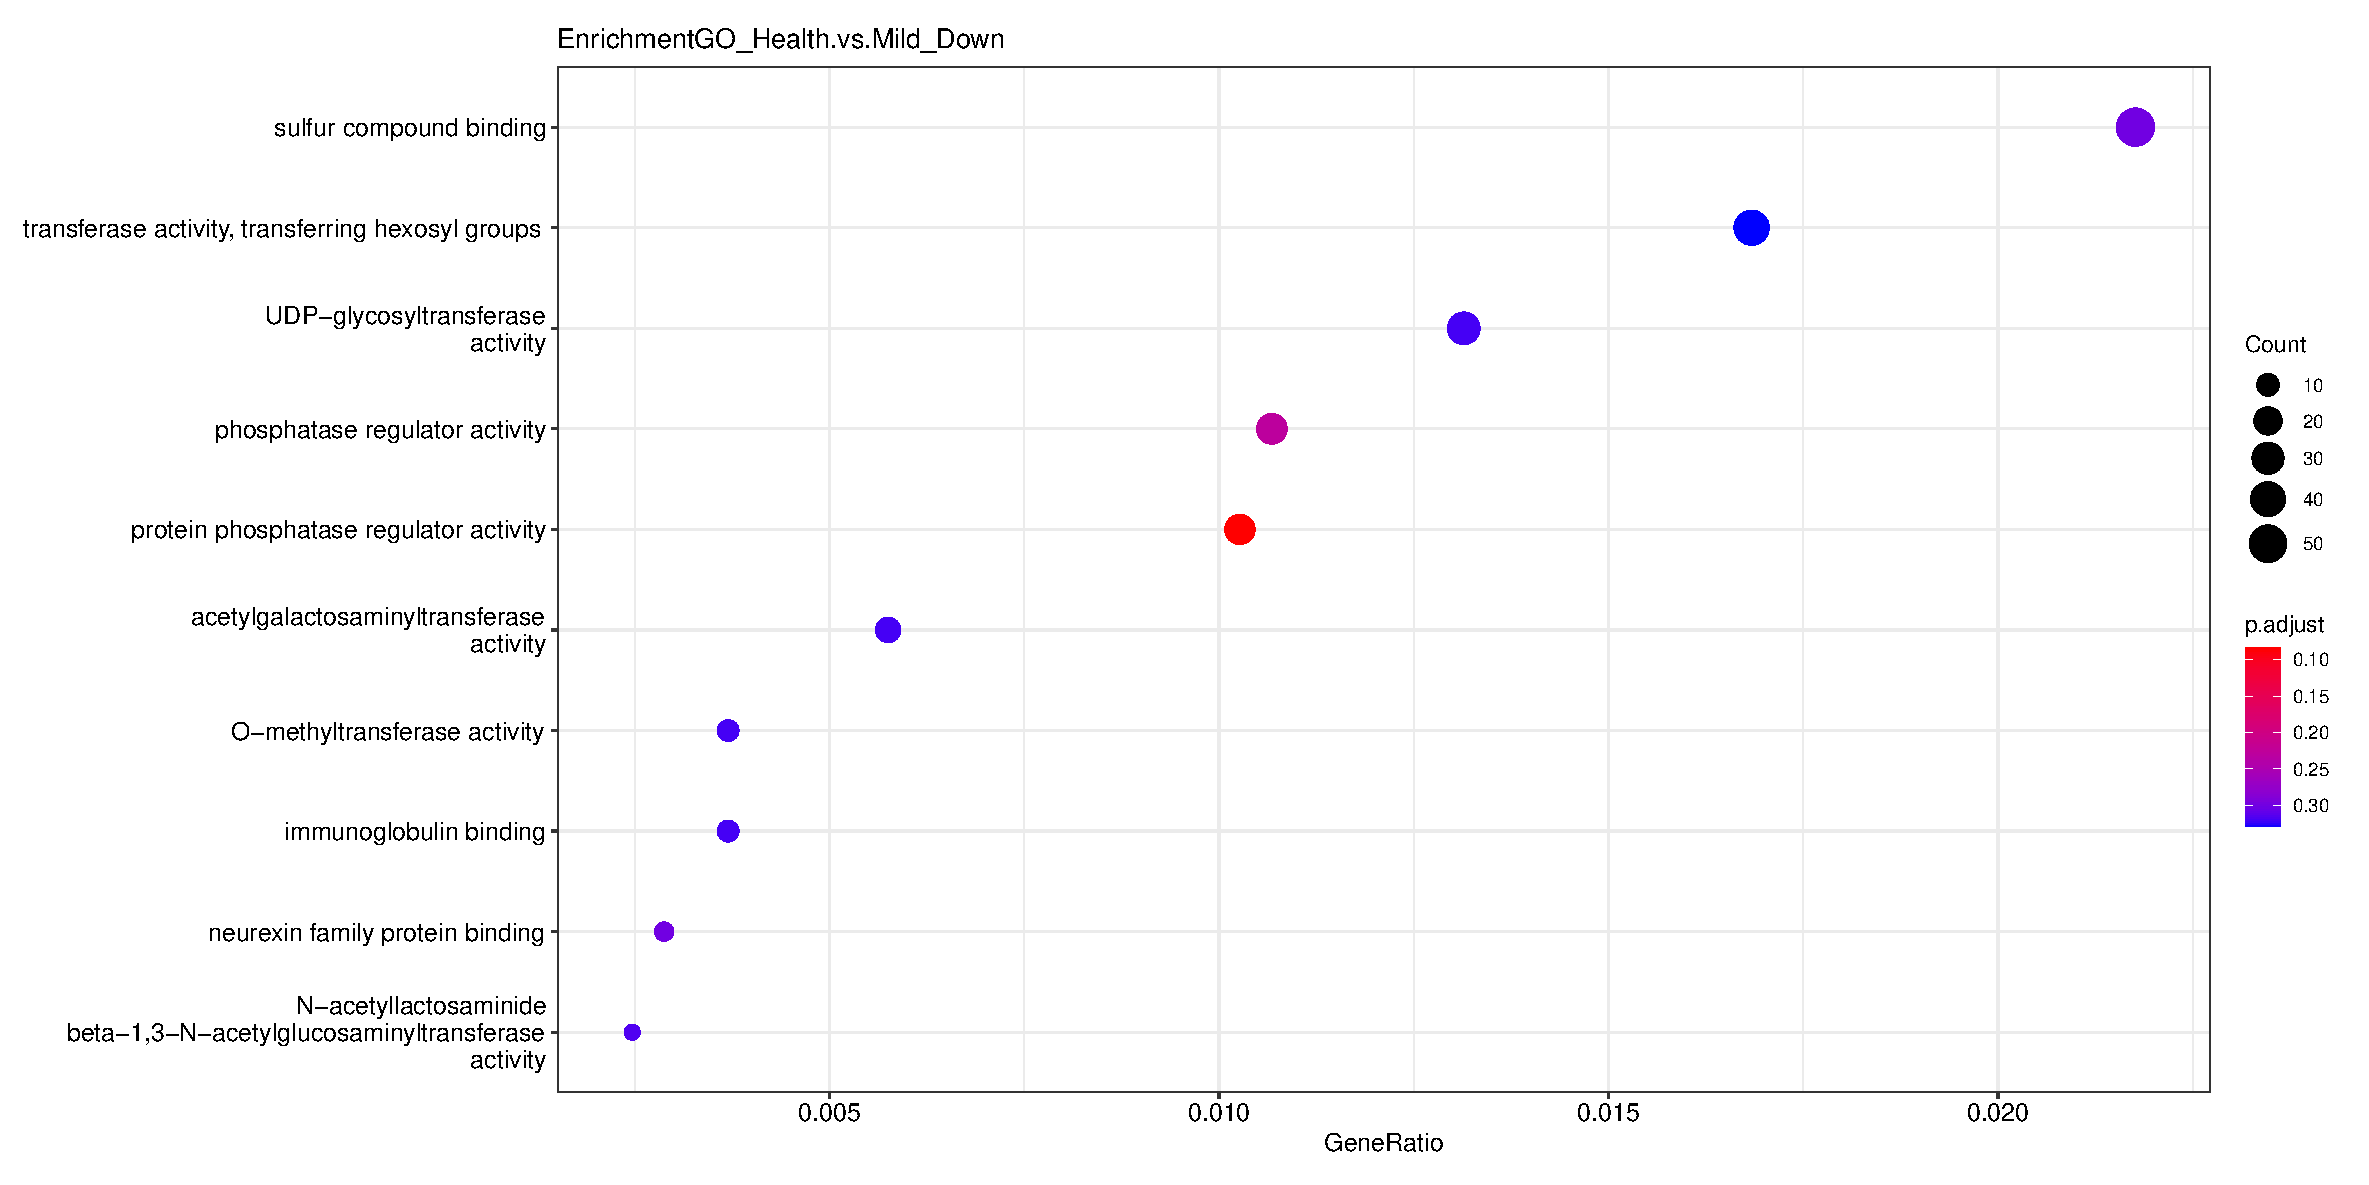
\includegraphics[width=.45\textwidth]{image/EGOHMD.eps}}
	\\
	\subfigure[healthy vs severe up genes] {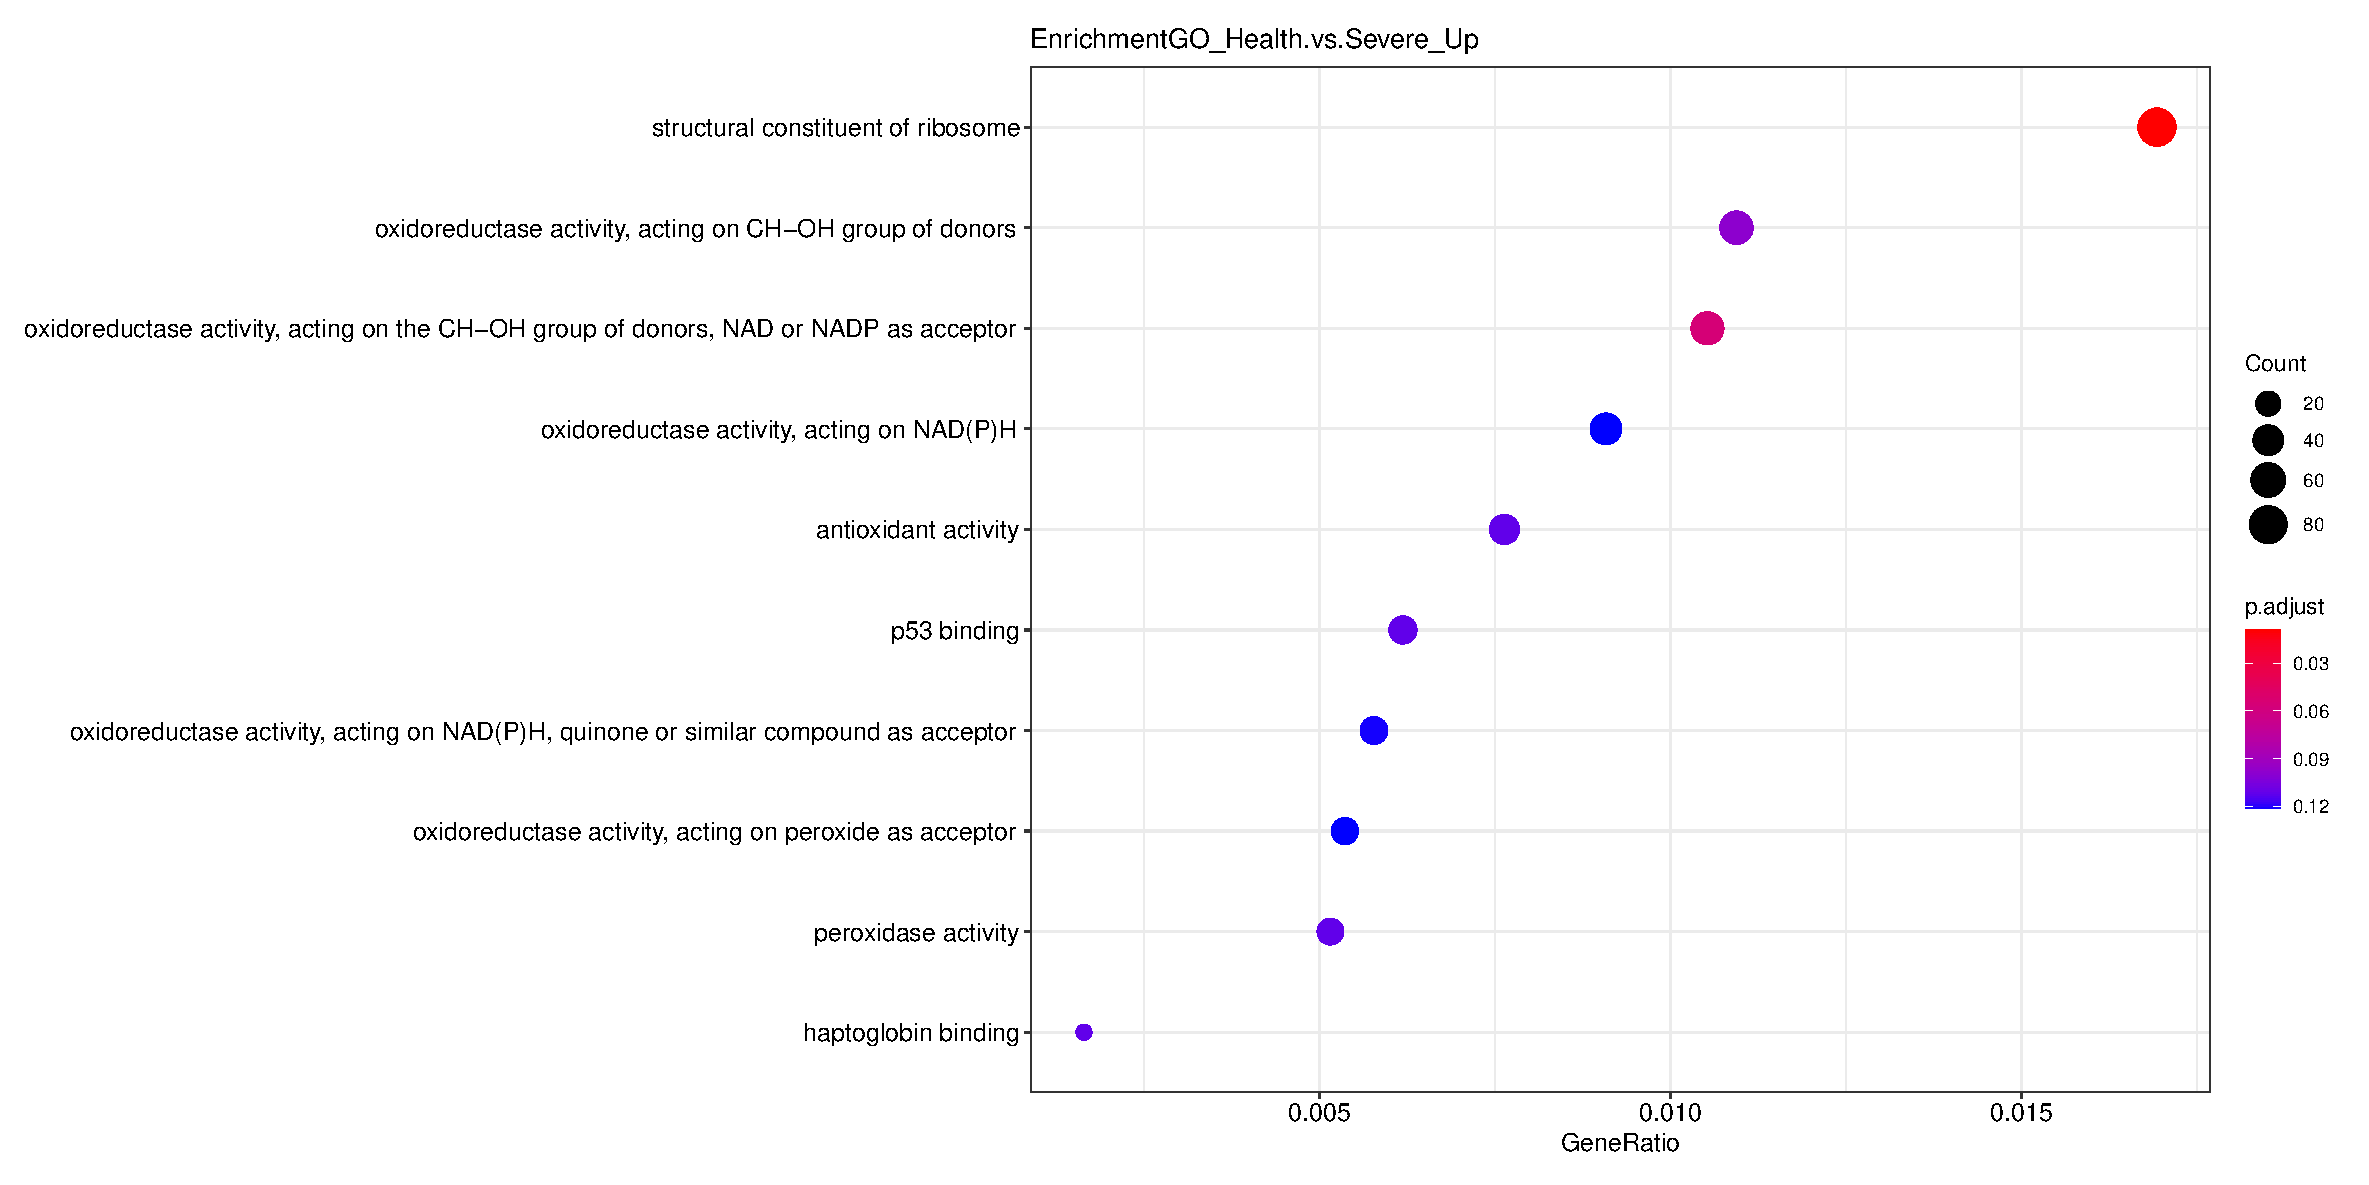
\includegraphics[width=.45\textwidth]{image/EGOHSU.eps}}
	\subfigure[healthy vs severe down genes] {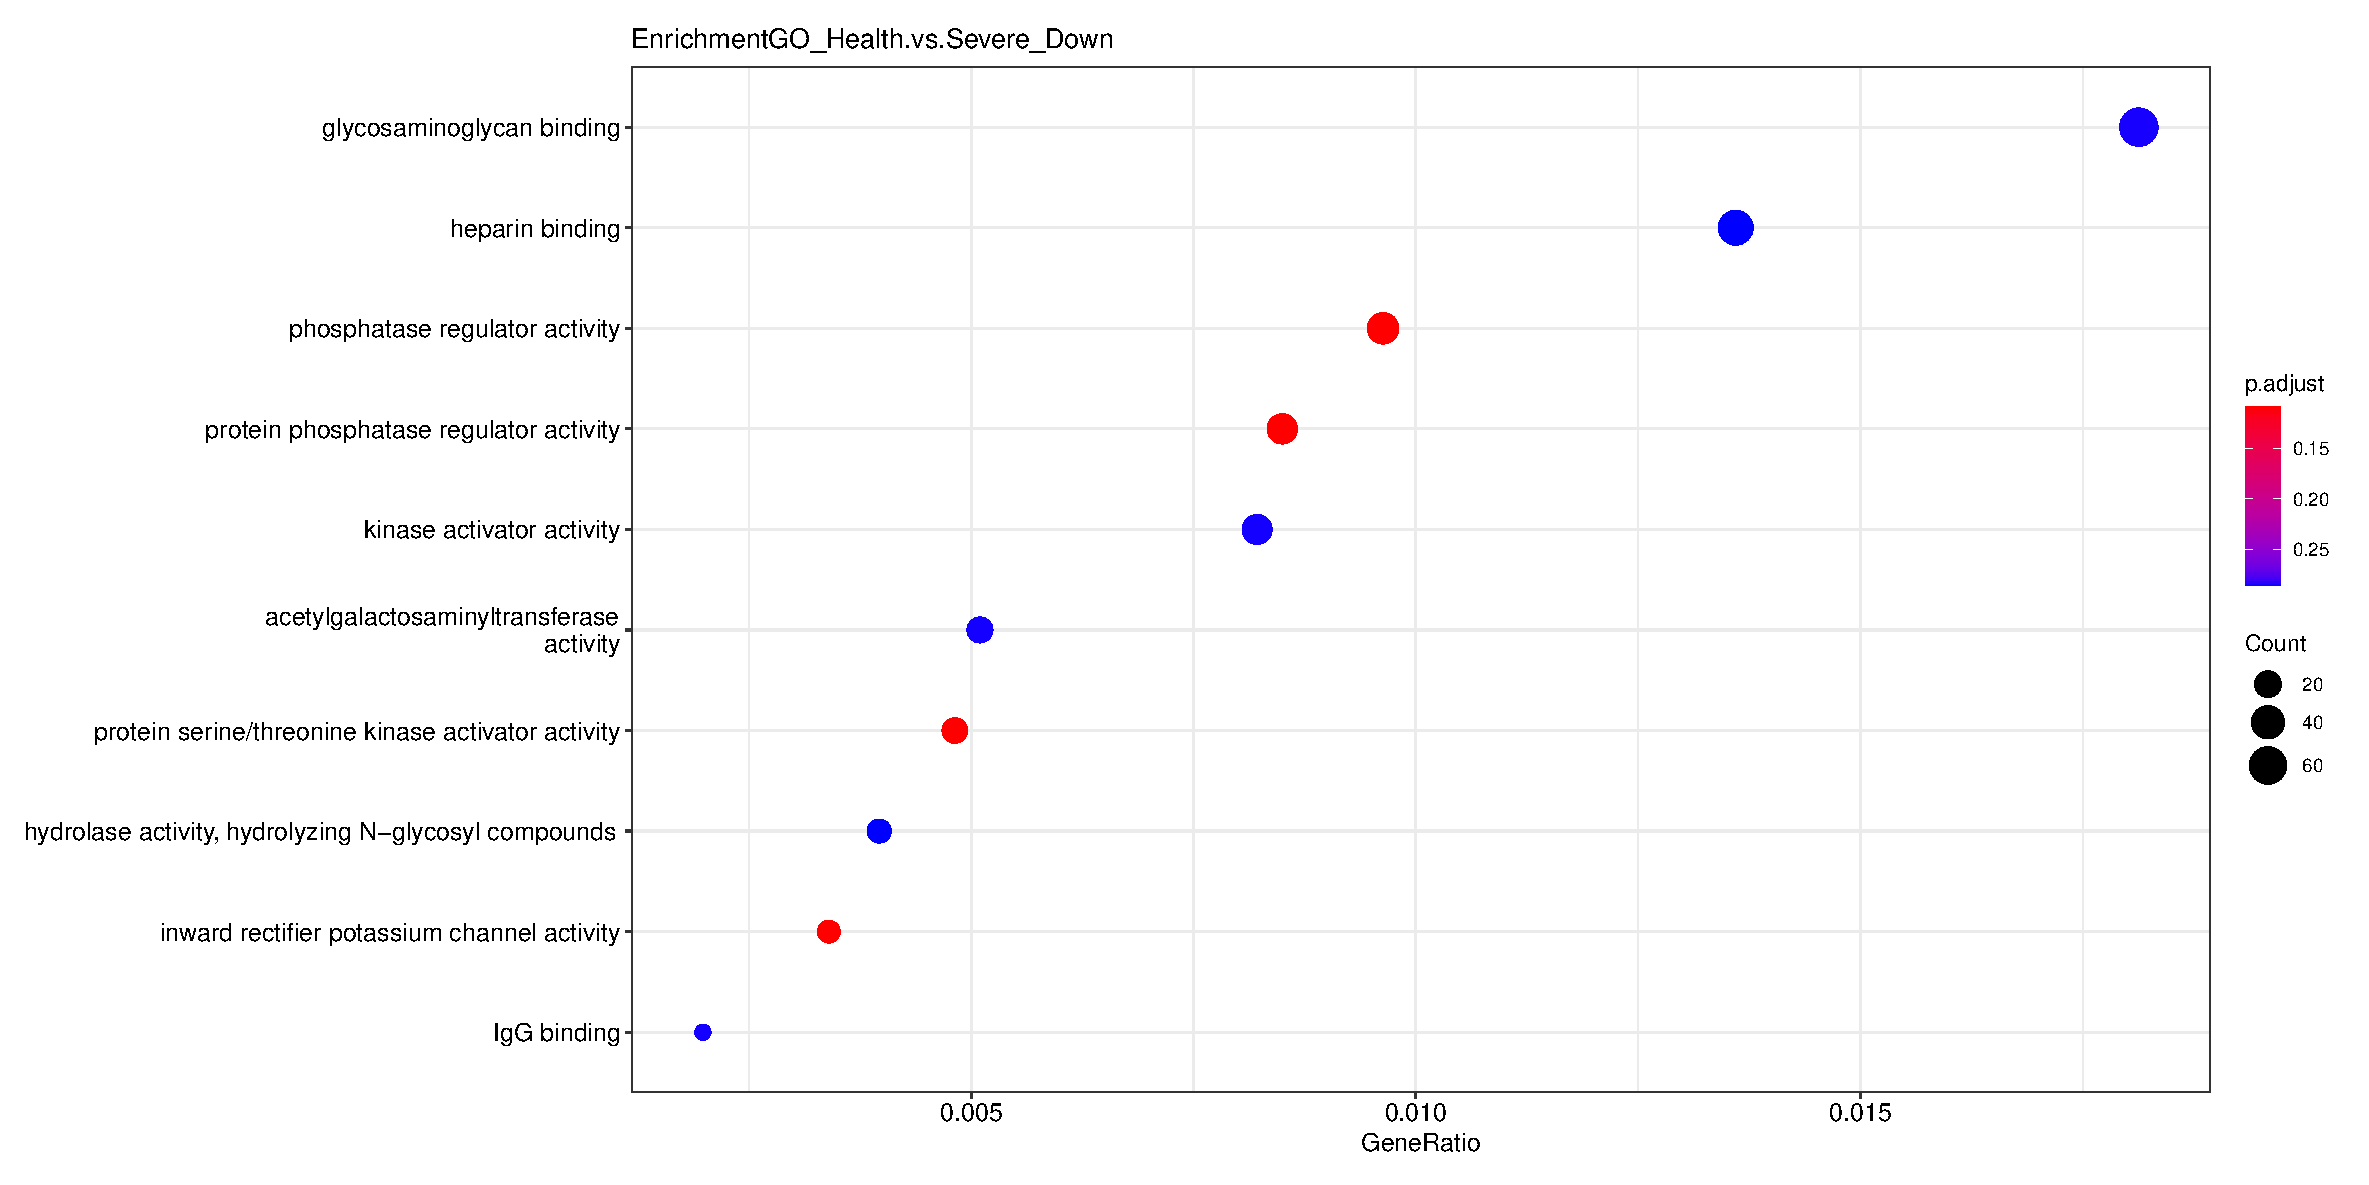
\includegraphics[width=.45\textwidth]{image/EGOHSD.eps}}
    \caption{GO Enrichment Results}
    \label{UMAP}
\end{figure}

\section{Discussion}
While the student wants to reproduce the procedures in the paper in Front. Immunol., on 18 February 2021, titled \textit{Inflammation and Antiviral Immune Response Associated With Severe Progression of COVID-19}\upcite{fimmu2021} , due to lack of detailed data processing protocols, the results cannot be exactly the same as the ones published in the original paper. However, most of the results in this report is consistent with the original paper, indicating that even with different methods, the conclusions drawn by the authors is solid to some extent.

The number of DEGs is slightly different from that in the paper, but the numbers are in the same magnitude. The PCA results indicates that the the healthy patients can be easily separated from infected ones, while the difference between mild and severe, is harder to tell.

According to the heat map, if all the genes are used, no significant difference can be seen, and the results by the clustering algorithm is not reasonable. However, if the top significant genes are selected to draw the heat map, significant difference can be seen, and the the clustering algorithm gives reasonable results.


\bibstyle{unsrt}
\bibliography{references}{}
\end{document}
